
\chapter{Experiments}

We attempt to decode progressively harder features of the music signal from the EEG recordings.
We utilize the preprocessing pipeline described in the previous section.
For the Bi-LSTM model, we skip the final band power extraction step and feed the filtered EEG signal directly to the network.

\section{Song name prediction}

We start with the task of predicting the song name of a listened-to song based on the EEG signal.
We split the MUSIN-G dataset into recordings of 12 subjects for training and the remaining 8 subjects for testing (for CNN, half of the test set serves as the validation set).
We then train a model to predict the song name from the EEG signal.
We achieve the below results for each variant of the tested model.
For the CNN model we provide the best result out of the few tested variants, described below.

\begin{table}[h]
  \centering
  \begin{tabular}{|l|c|}
    \hline
    \textbf{Model} & \textbf{Accuracy} \\
    \hline
    Random  &  0.0833  \\
    KNN     & 0.1374 \\
    SVM     & 0.1229 \\
    XGBoost & 0.1668 \\
    CNN (best)      & \textbf{0.1802} \\
    \hline
  \end{tabular}
  \caption{Song name prediction accuracy: subject-wise split.}
  \label{tab:song-prediction}
\end{table}


Our results are comparable to the study by Pandey et al.\cite{pandey}, in which researchers achieved 12.5\% mean subject accuracy (a random classifier gives \(  \frac{1}{12} = 0.08(3) \)).

We also tested how the number of parameters influences the model's performance. We kept the architecture and varied number of convolution channels. The results are shown below.

\begin{figure}[h]
  \centering
  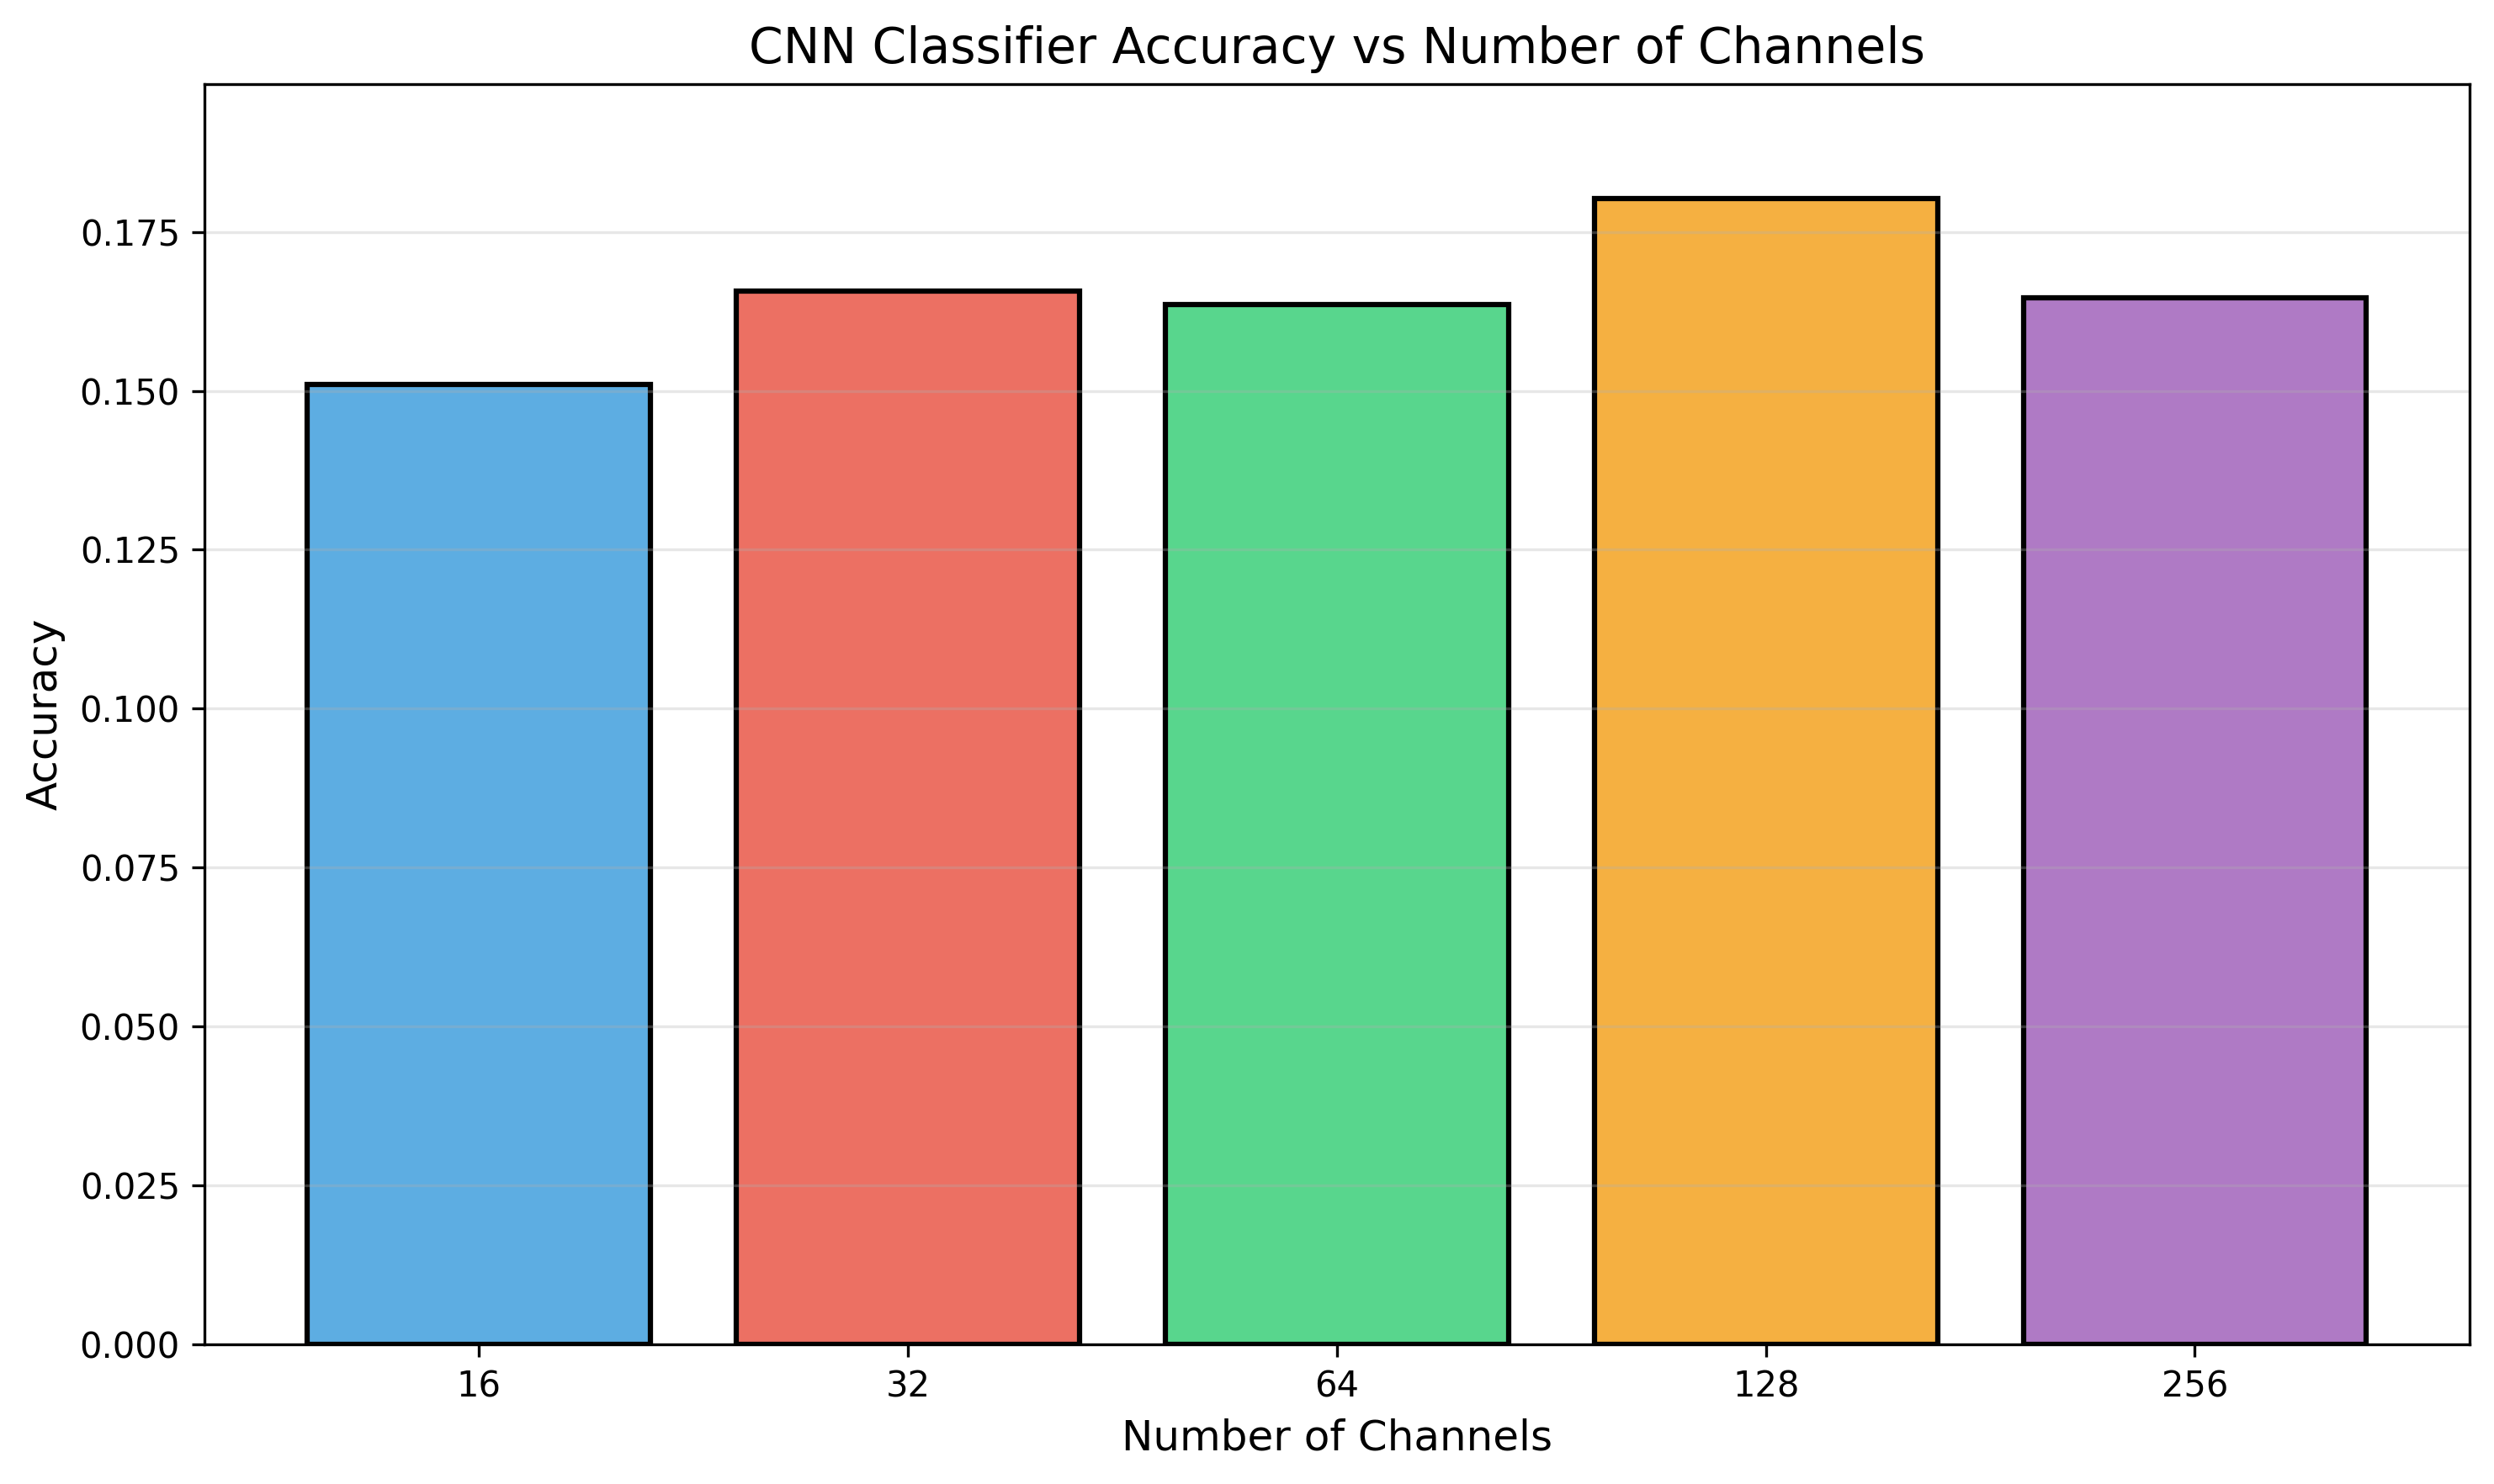
\includegraphics[width=0.7\linewidth]{imgs/cnn_channels_accuracy.png}
  \caption{CNN accuracy as a function of the number of convolution channels.}
  \label{fig:cnn-channels-accuracy}
\end{figure}


In the above study, researchers also tested scores achieved in a different testing paradigm. They split the MUSIN-G dataset into training and testing 
by taking the initial \( n \) seconds of each recording as training data and the remaining seconds as testing data. The study compares results that can be achieved for a few chosen \( n \) parameters (\(3, 5, 10, 20\)), achieving higher accuracy for larger training partitions.
The results in this variant of the experiment are much higher (\( 84\% \)) than in the previous variant.
We are able to reproduce these results, and for \( n=20 \) we achieve accuracies as shown in the table:

\begin{table}[h]
  \centering
  \begin{tabular}{|l|c|}
    \hline
    \textbf{Model} & \textbf{Accuracy} \\
    \hline
    XGBoost & \textbf{0.85} \\
    SVM     & 0.57 \\
    KNN     & 0.64 \\
    NN      & 0.72 \\
    \hline
  \end{tabular}
  \caption{Song id prediction accuracy in the MUSIN-G dataset: temporal split.}
  \label{tab:song-id-temporal-split}
\end{table}

While the best model in the trial-wise split variant achieves 0.85\% accuracy, the best model in subject-wise split variant achieves only 0.18\%.
This means that the model fails to learn neural patterns that generalize across subjects.
This poor generalization suggests that the model in this trial-wise variant does not pick up on neural correlates of the music but rather on some trial-specific aspects of the EEG recording.
We test the hypothesis with two experiments. 

First, we run a similar experiment on the BCMI-training dataset. The dataset contains from 144 up to 432 trials recorded for a single subject.
The recordings share the ``emotionality'' of the listened-to music, but no listened-to song repeats across the dataset as the songs are computer-generated for each trial.
We find that, similarly to the study, classifiers are able to predict the trial ID from the EEG signal with high accuracy. 
The results are shown in the below table.

\begin{table}[h]
  \centering
  \begin{tabular}{|l|c|}
    \hline
    \textbf{Model} & \textbf{Accuracy} \\
    \hline
    XGBoost & 0.78 \\
    SVM     & \textbf{0.91} \\
    KNN     & 0.88 \\
    CNN      & ---    \\
    \hline
  \end{tabular}
  \caption{Song id prediction experiment in the BCMI-training dataset.}
  % \caption{Song id prediction experiment in the single subject variant in the BCMI-training dataset.}
  \label{tab:song-id-single-subject}
\end{table}

\subsection{DTW-based trial id prediction}

Secondly, guided by the intuition that the classifiers notice directly repeatable patterns in the EEG signal between training and test sets and are not forced to generalize beyond that, we propose the following experiment.
We attempt to predict the trial ID using the DTW algorithm.

DTW in its most basic form is a method of measuring the distance between two time series by finding an optimal alignment between them.
Such an alignment is a match between points of one time series and points of the other time series that minimizes the sum of distances between matched points, 
starts and ends at the two matched ends of the two time series, and is monotonic in between. 

We employ a version of the algorithm called approximate-subsequence-DTW, described in the methods section.
The algorithm allows for calculation of alignment cost between some infixes of the two sequences.
We use it to compare a "similarity" of one sequence to another.
Running it on two EEG sequences, we find what is the longest fragment that approximately repeats across the two signals.
Matching a test trial with every trial from a training set and comparing the lengths of the matches, we can find the most similar trial and use it to assign a prediction.

For a single subject of the BCMI-training dataset, we predict the trial ID of a test trial by finding, across all training trials,
the one that scores the highest when calculating the approximate-subsequence-DTW distance between the test trial and the training trial.
We fit the cost allowance hyperparameter on the validation set and then test the accuracy of the method on the test set. 
The cost parameter specifies how much cummulative difference between the matched points of the two sequence we allow.
With this simple method we achieve 50.83\% test accuracy.
% Accuracy: 61/120 = 50.83%
The experiment is meant to showcase that such direct pattern matching is possible and therefore---it is possible for the model to learn it and rely on it greatly, with little generalization capability.

\section{Emotion prediction}

The BCMI-training dataset is made of computer-generated snippets of music. These musical snippets are tagged with emotionality labels, one of 9 possibilities arranged on Valence and Arousal axes.
To compare the difficulty of this task with previous tasks, we can think of emotionality labels as abstraction classes that join multiple individual trials together.
Therefore, it is easier to predict an emotion label than an identifier, as this requires less precision, but during training, the 
reward per training step is less valuable and gives less information.
The balance does not seem to be in favor of this task, as we are unable to achieve good results, even though we do in the prediction task.

\begin{table}[h]
\centering
\begin{tabular}{l c}
\hline
Method  & Accuracy \\
\hline
XGBoost & 0.1089 \\
SVM     & 0.1123 \\
KNN     & 0.1117 \\
CNN     & \textbf{0.1130} \\
\hline
\end{tabular}
\caption{Emotion prediction accuracy}
\label{tab:emotion-prediction}
\end{table}

\section{Music ``density'' prediction}

Looking for musical features visible through the EEG recording, we define a ``density'' of a music snippet and, by extension, the paired EEG snippet.
First, we mark note onsets in the music recordings. 
We do that by looking at the music's mel spectrograms and marking the time points at which the spectrogram's energy increases significantly, weighting the changes in the high frequencies more (High-Frequency-Content method).
The HFC method was visually compared to other methods and chosen as seemingly best.

\begin{figure}[h]
  \centering
  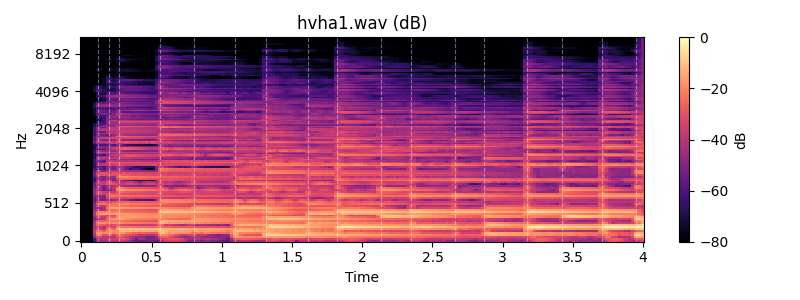
\includegraphics[width=\linewidth]{imgs/mel_onset_hvha1.wav.png}
  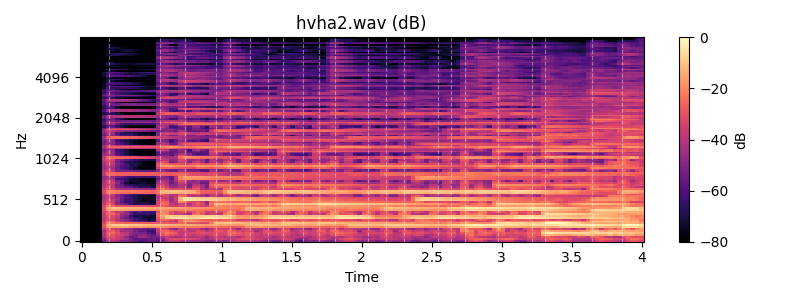
\includegraphics[width=\linewidth]{imgs/mel_onset_hvha2.wav.png}
  \caption{Spectrograms of two 4s music snippets with marked note onsets.}
  \label{fig:mel-onsets}
\end{figure}

Now, for a chosen length of a time window, we get a certain distribution of the number of note onsets within windows of this length.
Calculating the median number, we can split the snippets into two classes: the ``sparse'' class with a number of onsets below the median, and the ``dense'' class with a number of onsets above the median.
We calculate the median only on the training set and define a classification task of predicting the class of a snippet based on the paired EEG snippet.
We hope that success in this task may be a stronger indicator that some musical features are present and can be decoded from the EEG signal.

Results are shown in the table below.

\begin{table}[h]
  \centering
  \begin{tabular}{|l|c|}
    \hline
    \textbf{Model} & \textbf{Accuracy} \\
    \hline
    XGBoost & \textbf{0.5407} \\
    SVM     & 0.5093 \\
    KNN     & 0.5264 \\
    CNN     & 0.5206 \\
    \hline
  \end{tabular}
  \caption{Music density prediction accuracy.}
  \label{tab:density-prediction}
\end{table}

\section{Music reconstruction}

We attempt to reconstruct listened-to music from the EEG signal for the MUSIN-G dataset.
We treat this task as an extension of the song ID prediction task: if a model can learn to predict a song, can it learn to predict the specific fragment of a song and generate its mel spectrogram?
Our architecture of the $CNN_{reconstruction}$ model used for this task reflects this idea. 
It can be seen as an encoder and decoder model, with skip connections, where the encoder is similar to the $CNN_{classification}$ model.

Reflecting the results in the song identification tasks, we observe that the model is able to reconstruct music to some extent in the variant where 
single-subject recordings are split into training and test partitions by assigning the initial 20s of each recording to training.
The reconstructions are accurate enough to allow for meaningful classification (see figures below). 

In the cross-subject variant, where we investigate the ability for cross-subject generalization and a different portion of subjects is used for training and testing, 
we don't achieve any meaningful results in the reconstruction task. 
This matches the established accuracies in the song ID prediction task for this variant, which were much lower and were all between 12\% and 18\%, compared to the 57\% to 85\% range.


\begin{figure}[h]
  \centering
  \textbf{Accuracy scores in the temporal-split}
  \vspace{0.3cm}
  
  \begin{minipage}[t]{0.48\textwidth}
    \centering
    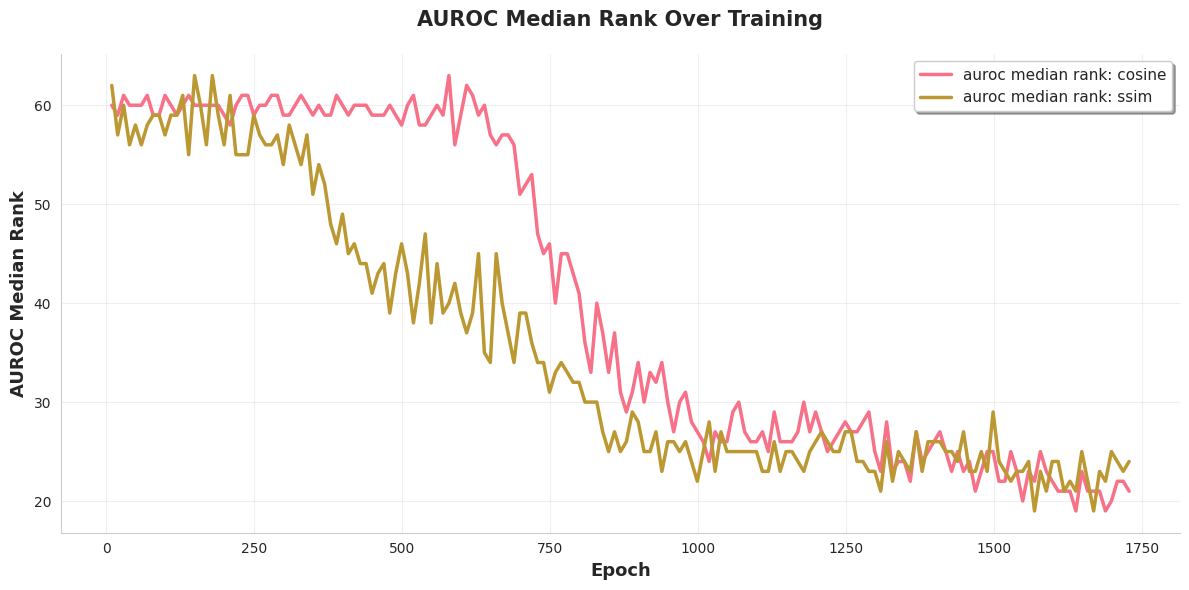
\includegraphics[width=\textwidth]{imgs/auroc_median_rank_plot.png}
    \caption{For a generated mel spectrogram, we calculate similarities with all 120 real spectrograms from the current batch. We then sort the spectrograms based on the similarity scores and find out what the rank of the true spectrogram is to assess the quality of our predicted one. The plot shows the median rank for two used similarity measures: cosine similarity and structural similarity.}
    \label{fig:auroc-median-rank}
  \end{minipage}
  \hfill
  \begin{minipage}[t]{0.48\textwidth}
    \centering
    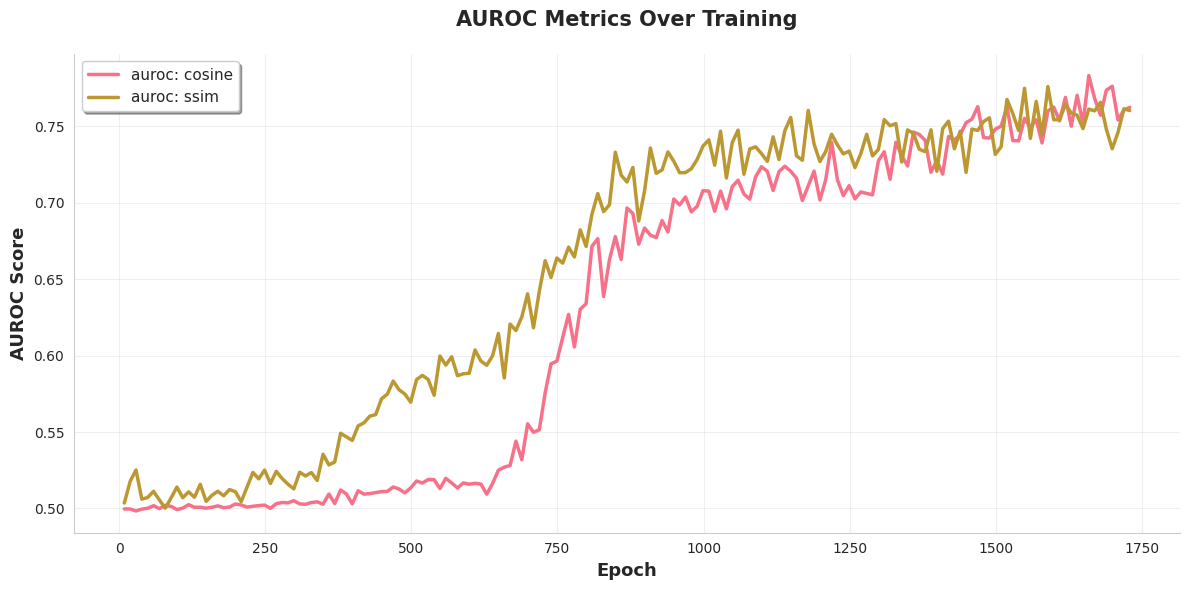
\includegraphics[width=\textwidth]{imgs/auroc_score_plot.png}
    \caption{AUROC score counts the ratio of times when the real spectrogram is ranked in the first half of the sorted order. It can be interpreted as the probability that the predicted spectrogram is closer to the real spectrogram than to a randomly sampled spectrogram.}
    \label{fig:auroc-score}
  \end{minipage}
\end{figure}


\begin{figure}[h]
  \centering
  \begin{tabular}{cc}
    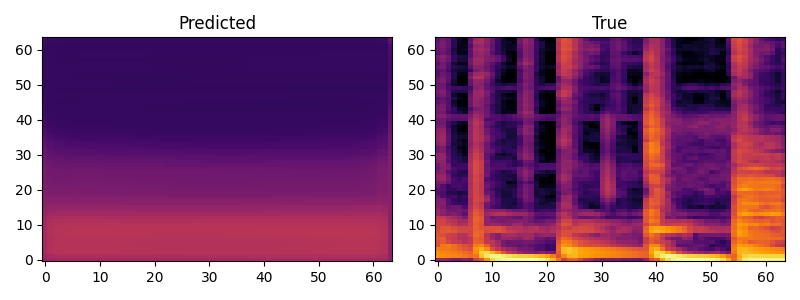
\includegraphics[width=0.48\textwidth]{imgs/spectrograms/media_images_val_spectrograms_8653_82c00f99e0bb079a497f.png} &
    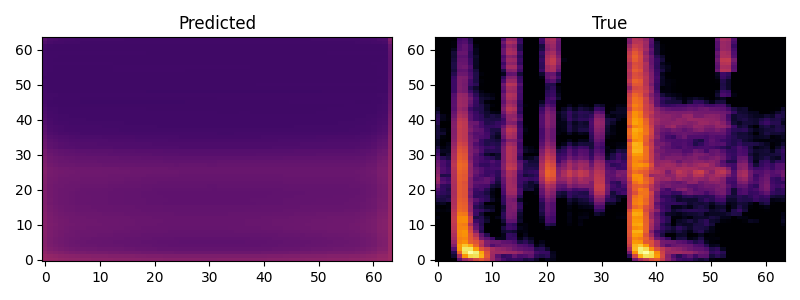
\includegraphics[width=0.48\textwidth]{imgs/spectrograms/media_images_val_spectrograms_8653_8c3ea155cfdde6d1ee92.png} \\
    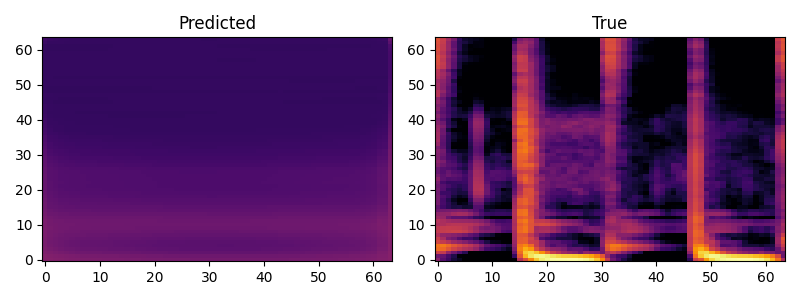
\includegraphics[width=0.48\textwidth]{imgs/spectrograms/media_images_val_spectrograms_8653_8fed809dd87da9f5b5f0.png} &
    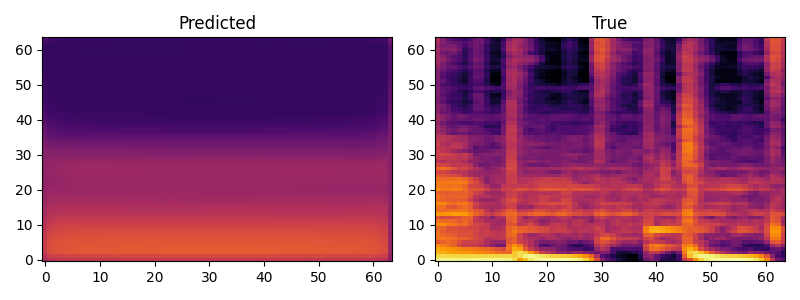
\includegraphics[width=0.48\textwidth]{imgs/spectrograms/media_images_val_spectrograms_8653_f0d90e1a1f7ae3ca67ea.png} \\
    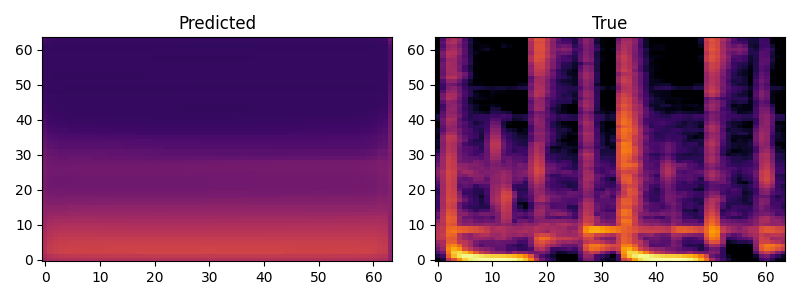
\includegraphics[width=0.48\textwidth]{imgs/spectrograms/media_images_val_spectrograms_8658_54ba5db2984c3817cb8d.png} &
    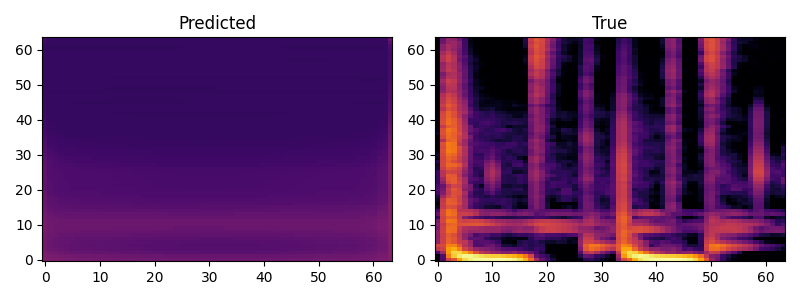
\includegraphics[width=0.48\textwidth]{imgs/spectrograms/media_images_val_spectrograms_8658_7942d7e56630eac823de.png} \\
    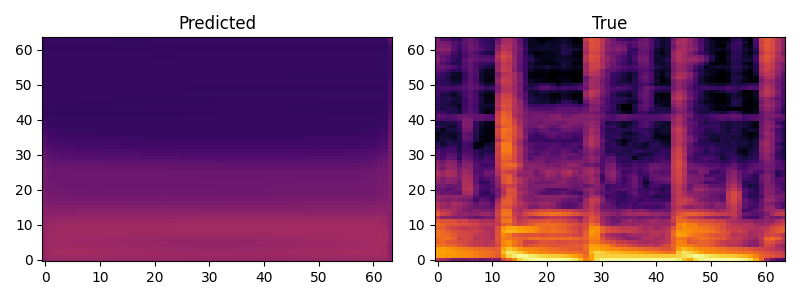
\includegraphics[width=0.48\textwidth]{imgs/spectrograms/media_images_val_spectrograms_8658_7baf70115b8f56210f30.png} &
    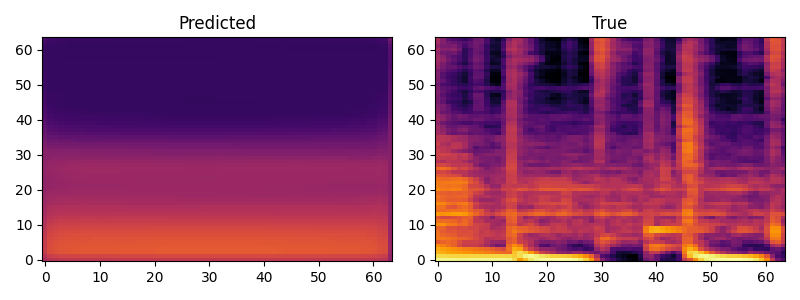
\includegraphics[width=0.48\textwidth]{imgs/spectrograms/media_images_val_spectrograms_8658_9f4076f20a86ba1957bf.png}
  \end{tabular}
  \caption{Reconstructed spectrograms.}
  \label{fig:reconstructed-spectrograms}
\end{figure}

Looking at the reconstructed spectrograms, we can notice that the network has not yet learned the high-resolution temporal aspects of the songs.
It cannot mark note onsets accurately. Instead, it tends to produce smooth spectrograms with almost equally colored rows that show the average power in a frequency band.

\subsection{Time-constant reconstruction}

To test the hypothesis that the network learns to reconstruct an averaged spectrogram for a music fragment, we train a simplified model.
The model has similar architecture to the main CNN model, but instead outputs an image of shape 64x1 which is then broadcasted to the desired shape of 64x64.
With this change we also don't need the full image decoder and therefore keep just a single fully connected layer.

The model is strictly less flexible, but we observe that the results achieved by it are not much worse than the results of the main model.
Comparing these results to the main model we observe few percentage points difference in AUROC scores.

\begin{figure}[h]
  \centering
  \textbf{Accuracy scores for time-constant reconstruction}
  \vspace{0.3cm}
  
  \begin{minipage}[t]{0.48\textwidth}
    \centering
    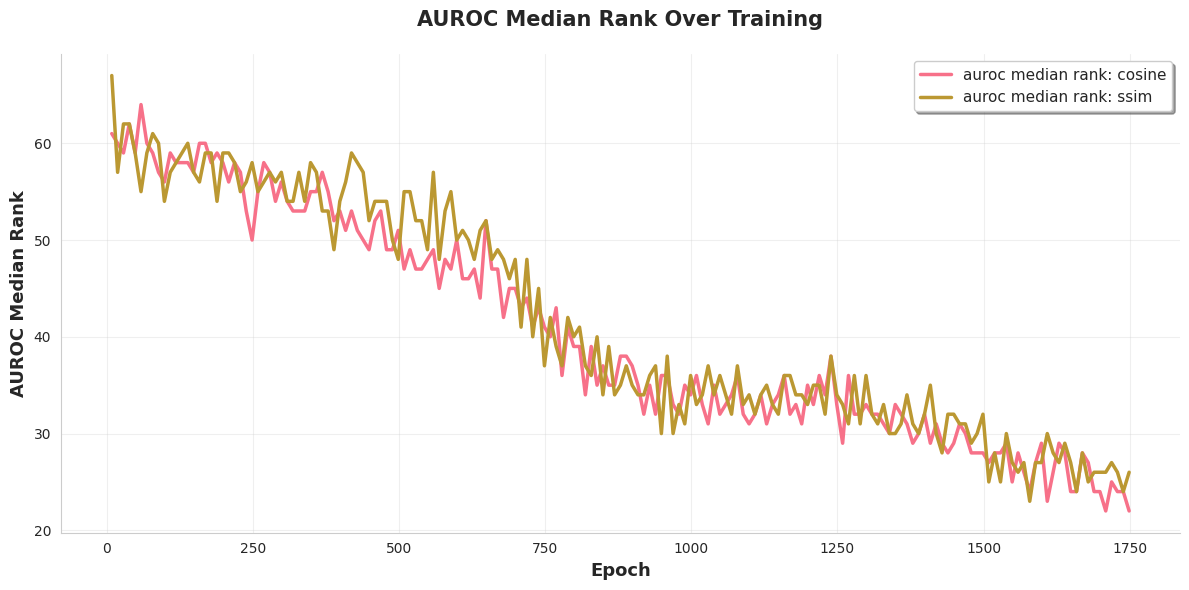
\includegraphics[width=\textwidth]{imgs/medianrank_timeconstant.png}
    \caption{Median rank comparison between the main model and the time-constant model. The time-constant model achieves similar performance despite its reduced flexibility.}
    \label{fig:medianrank-timeconstant}
  \end{minipage}
  \hfill
  \begin{minipage}[t]{0.48\textwidth}
    \centering
    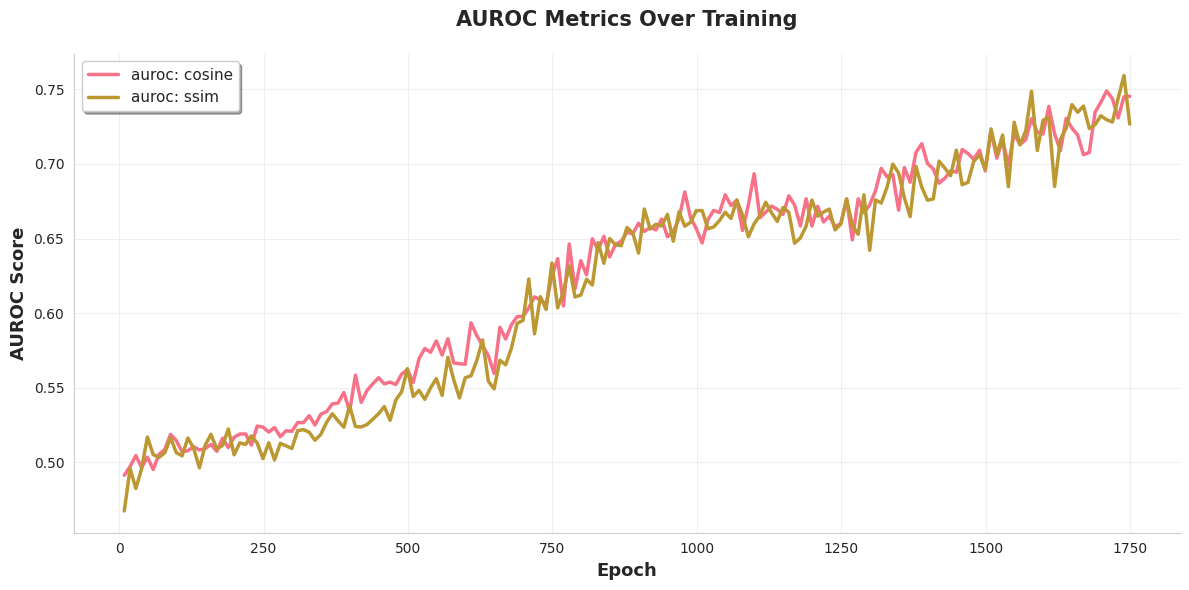
\includegraphics[width=\textwidth]{imgs/auroc_timeconstant.png}
    \caption{AUROC score comparison showing that the time-constant model performs comparably to the full model, supporting the hypothesis that the network learns averaged spectrograms.}
    \label{fig:auroc-timeconstant}
  \end{minipage}
\end{figure}

\begin{figure}[h]
  \centering
  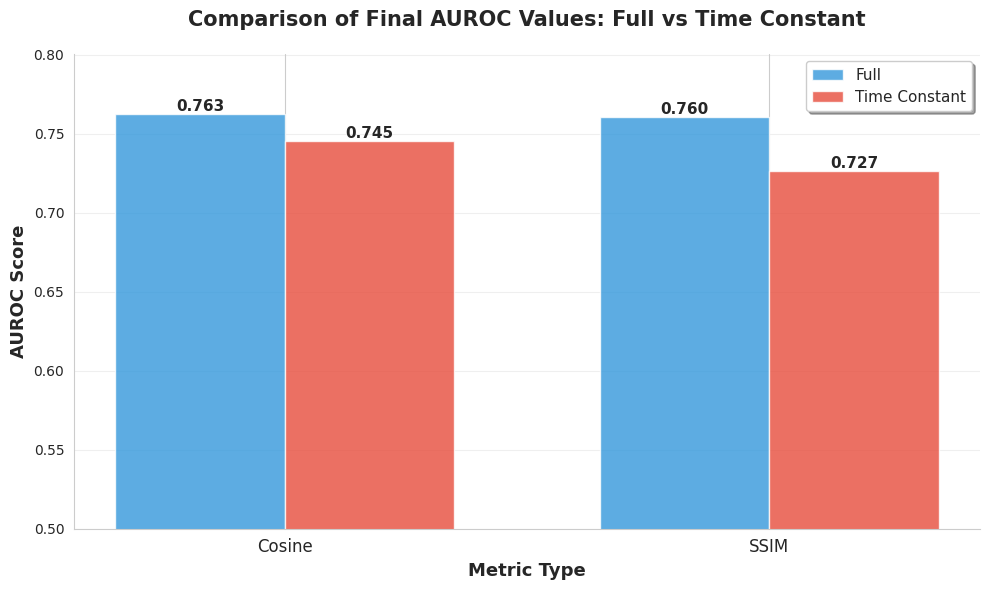
\includegraphics[width=0.7\textwidth]{imgs/auroc_comparison.png}
  \caption{AUROC comparison between the main reconstruction model and the time-constant model.}
  \label{fig:auroc-comparison}
\end{figure}

\section{Attempt at decoding rhytm}

Having decoded the harmonic content we look to rhytm.
The results of full reconstruction suggest that to decode rhytm we need to use different methods.
We take inspiration from \cite{daly} where a Bi-LSTM network is used to perform music decoding in waveform domain.
We aim to predict an onset detection function (ODF), which is a scalar function whose picks indicate sound onsets.
A target ODF is calculated using HFC method which responds to changes in the high frequency part of the spectrogram.
We trained the model on 3 different EEG data types: all 129 EEG channels, only 12 channels hand-picked as relevant to music processing and 12 preprocessed ICA channels.
Separate models are trained for subjects.
We assess quality of predictions by calculating AUROC scores similarly to the mel reconstruction case: we compute similarity to all other ODFs and rank them.

\begin{figure}[h]
  \centering
  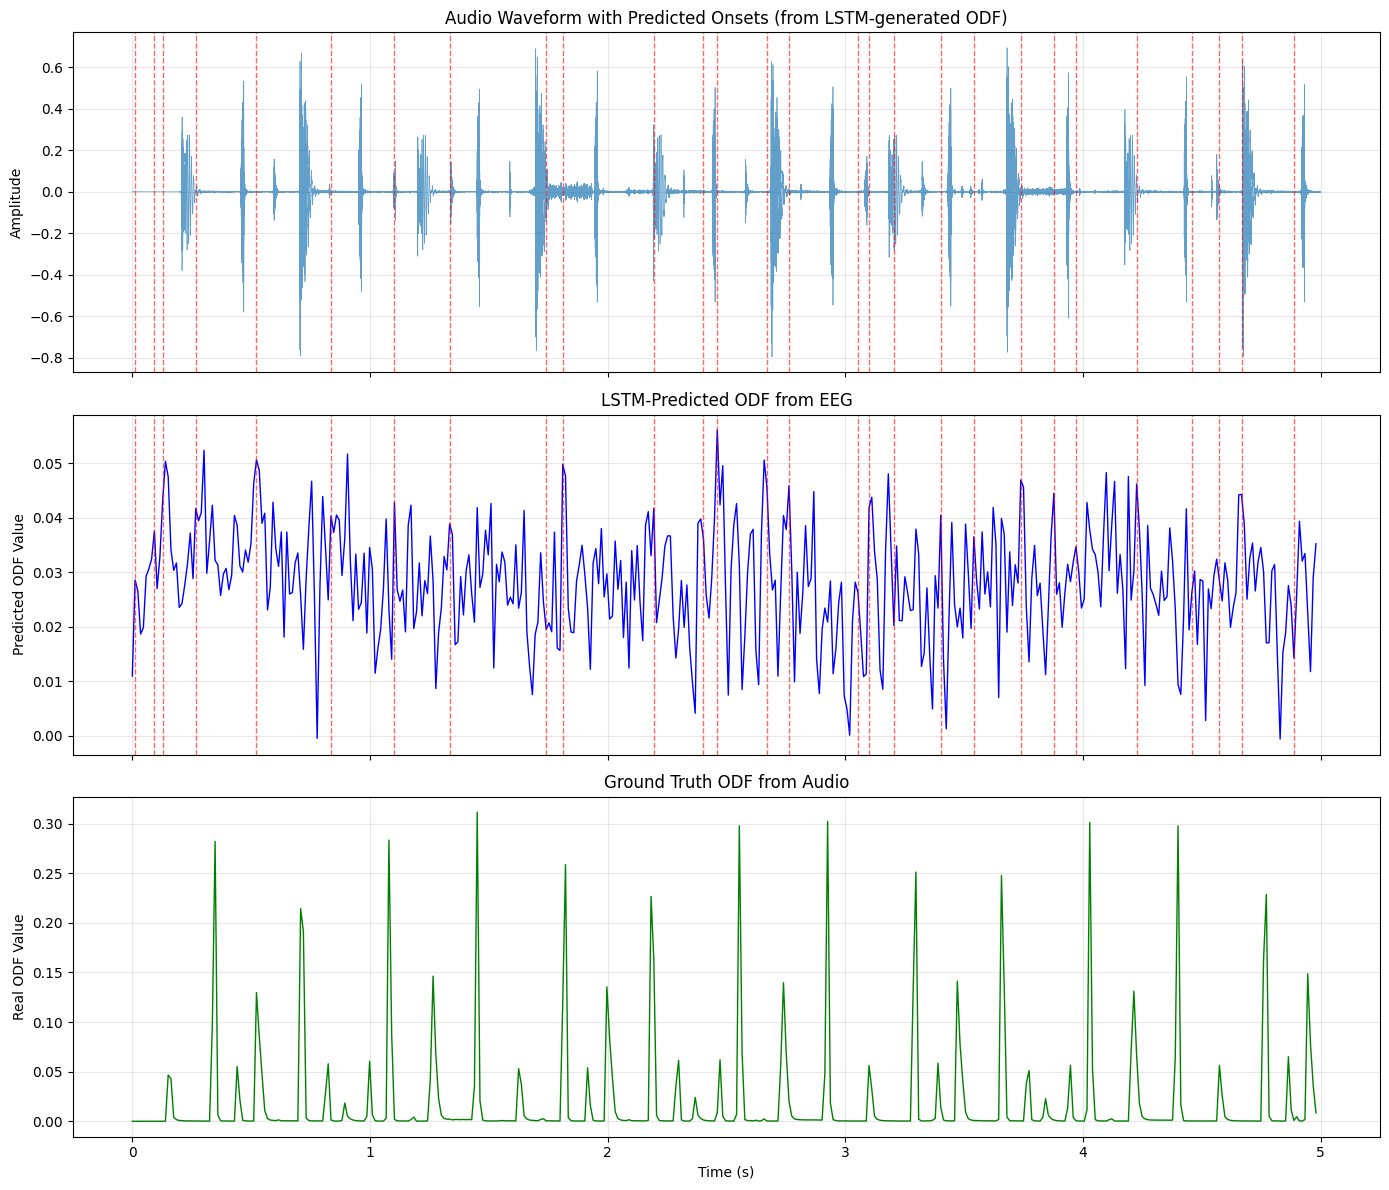
\includegraphics[width=\linewidth]{imgs/lstm_odf_plots.png}
  \caption{LSTM onset detection function plots.}
  \label{fig:lstm-odf-plots}
\end{figure}


In all variants, eventhough we observe training in loss, we do not observe significant results in AUROC scores. Inspecting the predictions visually leaves no doubt in failure of the method.
We also try to overfit the model on single trial, with similar lack of results.

\section{Conclusion and future work}

We had achieved varied success finding features decodable from music to be: song name and music density, but not emotion label. 
We can also reconstruct music in a form of spectrograms.

One could ponder about the use of transformers for below tasks, but we realize that we have unsufficient data to train such models.

% \section{EEG analysis}

% We use this preprocessing with these methods.

% potrzeba: "eeg wygląd", eeg spektrogram, pipeline diagram and pictures, graph acc/subject

% \section{Music id prediction}

% similar:
%  - https://arxiv.org/abs/2009.08793: cnn musin-g
%  - https://www.researchgate.net/publication/360792627_Music_Identification_Using_Brain_Responses_to_Initial_Snippets: 

% \subsection{on musing}

% \subsubsection{12 songs: 90\% }
% \subsubsection{generalization: 20\% }

% \subsection{on bcmi}

% potrzeba: wyniki